\PassOptionsToPackage{unicode=true}{hyperref} % options for packages loaded elsewhere
\PassOptionsToPackage{hyphens}{url}
\documentclass[10pt,ignorenonframetext,aspectratio=169]{beamer}
\setbeamertemplate{caption}[numbered]
\setbeamertemplate{caption label separator}{: }
\setbeamercolor{caption name}{fg=normal text.fg}
\beamertemplatenavigationsymbolsempty
\usepackage{lmodern}
\usepackage{amssymb,amsmath}
% Thanks, @Xyv
\usepackage{calc}
\usepackage{ifxetex,ifluatex}
\usepackage{fixltx2e} % provides \textsubscript
\ifnum 0\ifxetex 1\fi\ifluatex 1\fi=0 % if pdftex
  \usepackage[T1]{fontenc}
  \usepackage[utf8]{inputenc}
\else % if luatex or xelatex
  \ifxetex
    \usepackage{mathspec}
  \else
    \usepackage{fontspec}
\fi
\defaultfontfeatures{Ligatures=TeX,Scale=MatchLowercase}







\fi

  \usetheme[]{macquarie}



% A default size of 24 is set in beamerthememonash.sty




% use upquote if available, for straight quotes in verbatim environments
\IfFileExists{upquote.sty}{\usepackage{upquote}}{}
% use microtype if available
\IfFileExists{microtype.sty}{%
  \usepackage{microtype}
  \UseMicrotypeSet[protrusion]{basicmath} % disable protrusion for tt fonts
}{}


\newif\ifbibliography


\hypersetup{
      pdftitle={STAT 1378},
            pdfborder={0 0 0},
    breaklinks=true}
%\urlstyle{same}  % Use monospace font for urls




  \usepackage{color}
  \usepackage{fancyvrb}
  \newcommand{\VerbBar}{|}
  \newcommand{\VERB}{\Verb[commandchars=\\\{\}]}
  \DefineVerbatimEnvironment{Highlighting}{Verbatim}{commandchars=\\\{\}}
  % Add ',fontsize=\small' for more characters per line
  \usepackage{framed}
  \definecolor{shadecolor}{RGB}{248,248,248}
  \newenvironment{Shaded}{\begin{snugshade}}{\end{snugshade}}
  \newcommand{\AlertTok}[1]{\textcolor[rgb]{0.94,0.16,0.16}{#1}}
  \newcommand{\AnnotationTok}[1]{\textcolor[rgb]{0.56,0.35,0.01}{\textbf{\textit{#1}}}}
  \newcommand{\AttributeTok}[1]{\textcolor[rgb]{0.77,0.63,0.00}{#1}}
  \newcommand{\BaseNTok}[1]{\textcolor[rgb]{0.00,0.00,0.81}{#1}}
  \newcommand{\BuiltInTok}[1]{#1}
  \newcommand{\CharTok}[1]{\textcolor[rgb]{0.31,0.60,0.02}{#1}}
  \newcommand{\CommentTok}[1]{\textcolor[rgb]{0.56,0.35,0.01}{\textit{#1}}}
  \newcommand{\CommentVarTok}[1]{\textcolor[rgb]{0.56,0.35,0.01}{\textbf{\textit{#1}}}}
  \newcommand{\ConstantTok}[1]{\textcolor[rgb]{0.00,0.00,0.00}{#1}}
  \newcommand{\ControlFlowTok}[1]{\textcolor[rgb]{0.13,0.29,0.53}{\textbf{#1}}}
  \newcommand{\DataTypeTok}[1]{\textcolor[rgb]{0.13,0.29,0.53}{#1}}
  \newcommand{\DecValTok}[1]{\textcolor[rgb]{0.00,0.00,0.81}{#1}}
  \newcommand{\DocumentationTok}[1]{\textcolor[rgb]{0.56,0.35,0.01}{\textbf{\textit{#1}}}}
  \newcommand{\ErrorTok}[1]{\textcolor[rgb]{0.64,0.00,0.00}{\textbf{#1}}}
  \newcommand{\ExtensionTok}[1]{#1}
  \newcommand{\FloatTok}[1]{\textcolor[rgb]{0.00,0.00,0.81}{#1}}
  \newcommand{\FunctionTok}[1]{\textcolor[rgb]{0.00,0.00,0.00}{#1}}
  \newcommand{\ImportTok}[1]{#1}
  \newcommand{\InformationTok}[1]{\textcolor[rgb]{0.56,0.35,0.01}{\textbf{\textit{#1}}}}
  \newcommand{\KeywordTok}[1]{\textcolor[rgb]{0.13,0.29,0.53}{\textbf{#1}}}
  \newcommand{\NormalTok}[1]{#1}
  \newcommand{\OperatorTok}[1]{\textcolor[rgb]{0.81,0.36,0.00}{\textbf{#1}}}
  \newcommand{\OtherTok}[1]{\textcolor[rgb]{0.56,0.35,0.01}{#1}}
  \newcommand{\PreprocessorTok}[1]{\textcolor[rgb]{0.56,0.35,0.01}{\textit{#1}}}
  \newcommand{\RegionMarkerTok}[1]{#1}
  \newcommand{\SpecialCharTok}[1]{\textcolor[rgb]{0.00,0.00,0.00}{#1}}
  \newcommand{\SpecialStringTok}[1]{\textcolor[rgb]{0.31,0.60,0.02}{#1}}
  \newcommand{\StringTok}[1]{\textcolor[rgb]{0.31,0.60,0.02}{#1}}
  \newcommand{\VariableTok}[1]{\textcolor[rgb]{0.00,0.00,0.00}{#1}}
  \newcommand{\VerbatimStringTok}[1]{\textcolor[rgb]{0.31,0.60,0.02}{#1}}
  \newcommand{\WarningTok}[1]{\textcolor[rgb]{0.56,0.35,0.01}{\textbf{\textit{#1}}}}



% From {rticles}
\newlength{\csllabelwidth}
\setlength{\csllabelwidth}{3em}
\newlength{\cslhangindent}
\setlength{\cslhangindent}{1.5em}
% for Pandoc 2.8 to 2.10.1
\newenvironment{cslreferences}%
  {}%
  {\par}
% For Pandoc 2.11+
\newenvironment{CSLReferences}[3] % #1 hanging-ident, #2 entry spacing
 {% don't indent paragraphs
  \setlength{\parindent}{0pt}
  % turn on hanging indent if param 1 is 1
  \ifodd #1 \everypar{\setlength{\hangindent}{\cslhangindent}}\ignorespaces\fi
  % set entry spacing
  \ifnum #2 > 0
  \setlength{\parskip}{#2\baselineskip}
  \fi
 }%
 {}
\usepackage{calc} % for calculating minipage widths
\newcommand{\CSLBlock}[1]{#1\hfill\break}
\newcommand{\CSLLeftMargin}[1]{\parbox[t]{\csllabelwidth}{#1}}
\newcommand{\CSLRightInline}[1]{\parbox[t]{\linewidth - \csllabelwidth}{#1}}
\newcommand{\CSLIndent}[1]{\hspace{\cslhangindent}#1}



% Prevent slide breaks in the middle of a paragraph:
\widowpenalties 1 10000
\raggedbottom

  \AtBeginPart{
    \let\insertpartnumber\relax
    \let\partname\relax
    \frame{\partpage}
  }
  \AtBeginSection{
    \ifbibliography
    \else
      \let\insertsectionnumber\relax
      \let\sectionname\relax
      \frame[plain]{\sectionpage}
    \fi
  }
  \AtBeginSubsection{
    \let\insertsubsectionnumber\relax
      \let\subsectionname\relax
      \frame[plain]{\sectionpage}
  }



\setlength{\parindent}{0pt}
\setlength{\parskip}{6pt plus 2pt minus 1pt}
\setlength{\emergencystretch}{3em}  % prevent overfull lines
\providecommand{\tightlist}{%
  \setlength{\itemsep}{0pt}\setlength{\parskip}{0pt}}

  \setcounter{secnumdepth}{0}




% Redefine shaded environment if it exists (to ensure text is black)
\ifcsname Shaded\endcsname
  \definecolor{shadecolor}{RGB}{225,225,225}
  \renewenvironment{Shaded}{\color{black}\begin{snugshade}\color{black}}{\end{snugshade}}
\fi
%%

  \title[]{STAT 1378}

  \subtitle{Assignment 3: Investigation of top 500 passwords.}



\date[
      02 November 2021
  ]{
      02 November 2021
        }

\begin{document}

% Hide progress bar and footline on titlepage
  \begin{frame}[plain]
  \titlepage
  \end{frame}



\begin{frame}{Main Investigation}
\protect\hypertarget{main-investigation}{}
\begin{itemize}
\tightlist
\item
  Investigation of top 500 passwords.
\item
  2 main questions:
\item
  Which Category has the weakest passwords?
\item
  Does having a stronger password affect how long it takes to crack it?
\item
  Finals Conclusions.
\item
  Other Recommendations.
\item
  References
\end{itemize}
\end{frame}

\begin{frame}{My Data:}
\protect\hypertarget{my-data}{}
Variables:

\begin{enumerate}
\tightlist
\item
  \alert{Rank} (Which is the most COMMON password)
\item
  \alert{Password} (The password itself).
\item
  \alert{Value} (Time to crack by online guessing)
\item
  \alert{TimeUnit} (The metric of time for a password brute force.)
\item
  \alert{OfflineCrackSec} (The amount of seconds for a password to be
  cracked)
\item
  \alert{Strength} (Strength of password according to security.org)
\item
  \alert{Font size}
\end{enumerate}
\end{frame}

\begin{frame}{Hypothesis:}
\protect\hypertarget{hypothesis}{}
\begin{enumerate}
\tightlist
\item
  Most exploitable category are names.
\item
  Name will have the shortest time to be cracked.
\item
  There IS a relationship between rank and strength
\item
  There is a correlation between strength and value
\end{enumerate}
\end{frame}

\hypertarget{datasets}{%
\section{Datasets}\label{datasets}}

\begin{frame}{Most Exploitable Category.}
\protect\hypertarget{most-exploitable-category.}{}
\begin{center}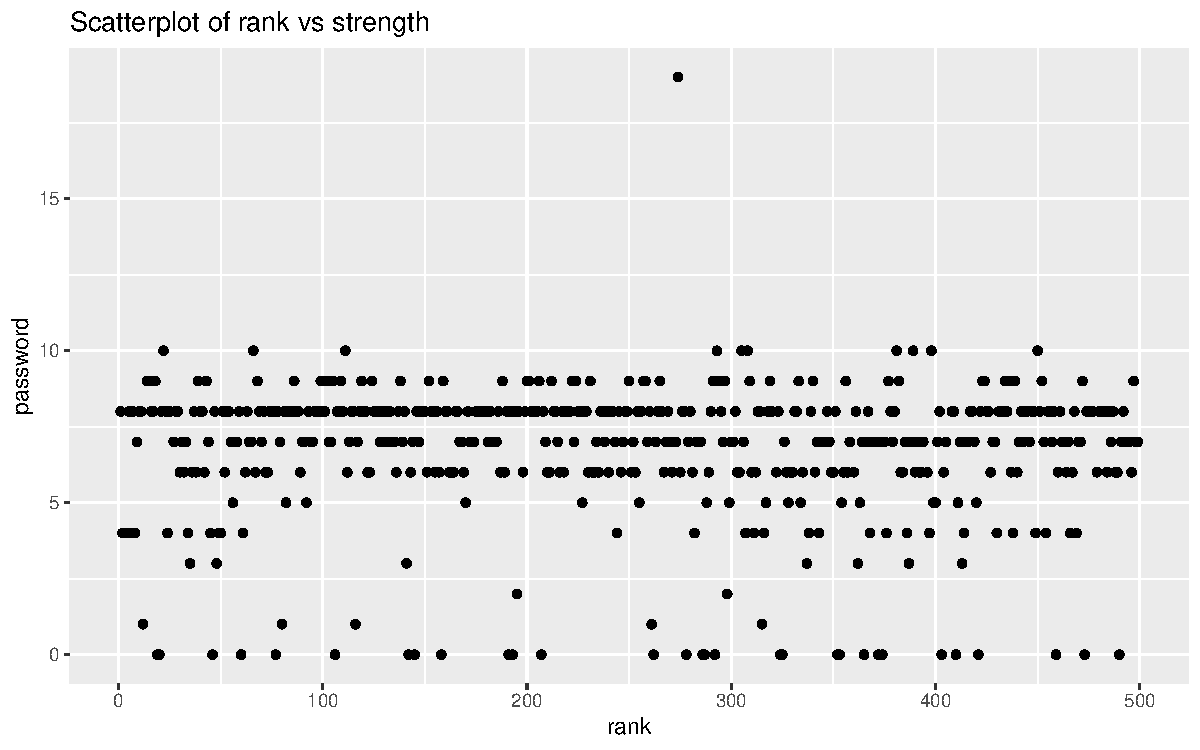
\includegraphics[width=0.8\linewidth]{Untitled_files/figure-beamer/unnamed-chunk-1-1} \end{center}
\end{frame}

\begin{frame}{Cateogry of the strongest and weakest passwords.}
\protect\hypertarget{cateogry-of-the-strongest-and-weakest-passwords.}{}
\begin{center}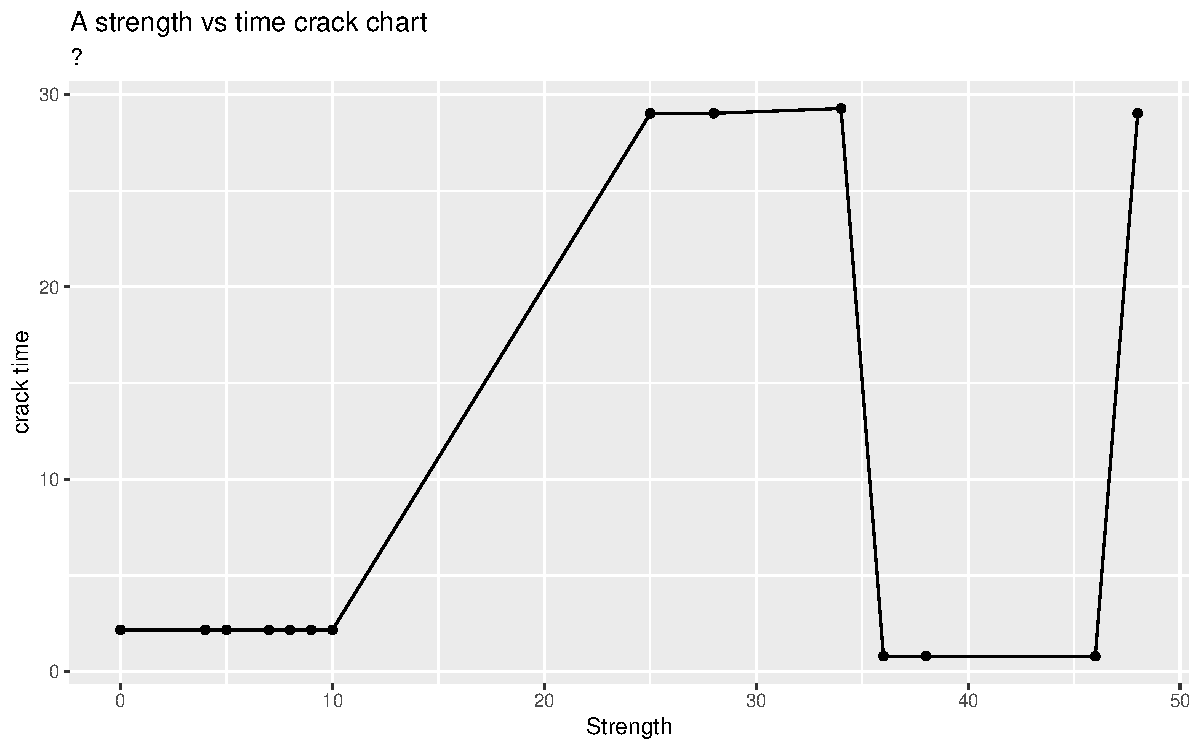
\includegraphics[width=0.8\linewidth]{Untitled_files/figure-beamer/plot2-1} \end{center}
\end{frame}

\begin{frame}{Category of the strength vs time to crack in s}
\protect\hypertarget{category-of-the-strength-vs-time-to-crack-in-s}{}
\begin{center}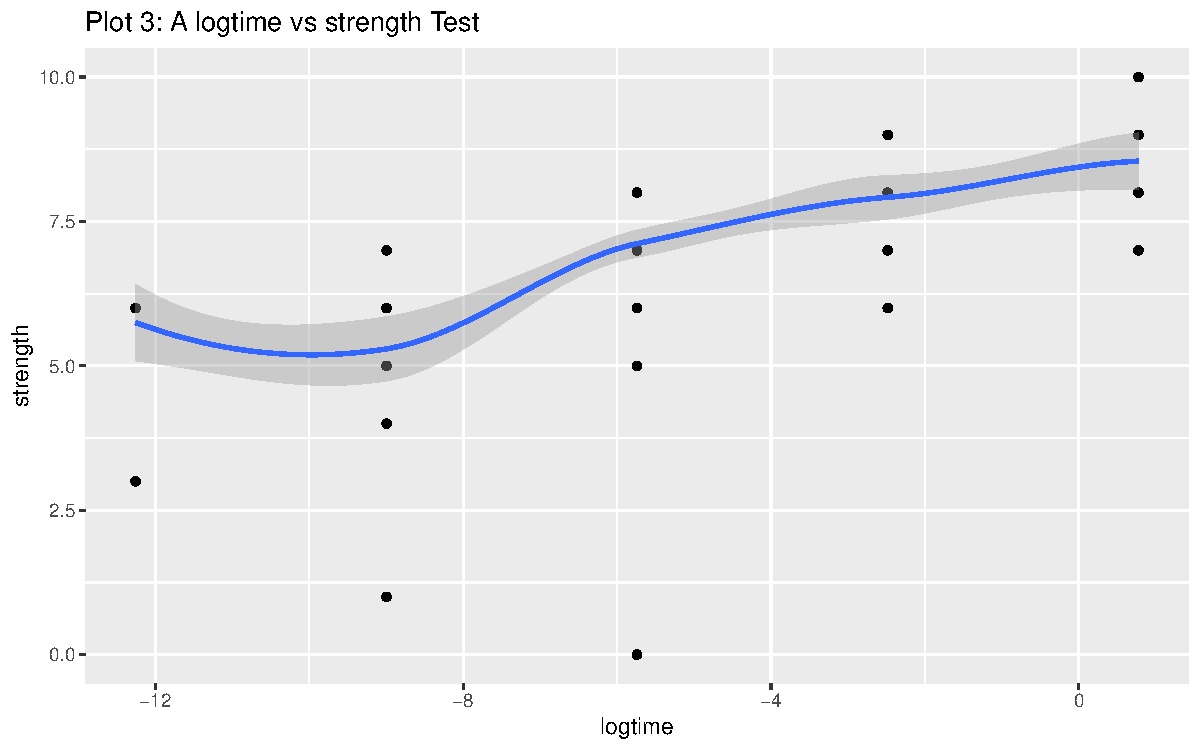
\includegraphics[width=0.8\linewidth]{Untitled_files/figure-beamer/plot2a-1} \end{center}
\end{frame}

\begin{frame}{Rank vs Strength ScatterPlot}
\protect\hypertarget{rank-vs-strength-scatterplot}{}
\begin{center}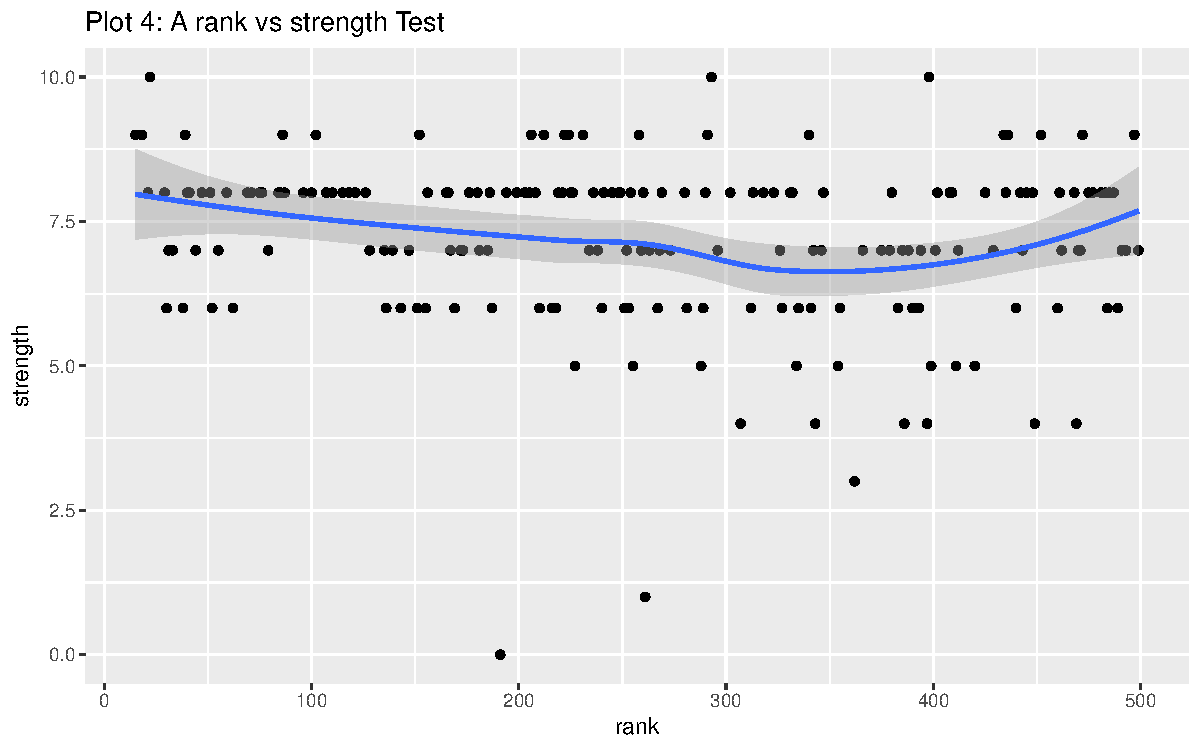
\includegraphics[width=0.8\linewidth]{Untitled_files/figure-beamer/plot3d-1} \end{center}
\end{frame}

\hypertarget{correlation-test}{%
\section{Correlation Test}\label{correlation-test}}

\begin{frame}[fragile]{Correlation Test}
\begin{Shaded}
\begin{Highlighting}[]
\NormalTok{correlation }\OtherTok{\textless{}{-}} \FunctionTok{cor}\NormalTok{(}\AttributeTok{x =}\NormalTok{ passwordsFiltered}\SpecialCharTok{$}\NormalTok{rank, }\AttributeTok{y =}\NormalTok{ passwordsFiltered}\SpecialCharTok{$}\NormalTok{strength)}

\NormalTok{correlation}
\end{Highlighting}
\end{Shaded}

\begin{verbatim}
## [1] 0.0466191
\end{verbatim}
\end{frame}

\begin{frame}{Value vs Strength Scatter plot.}
\protect\hypertarget{value-vs-strength-scatter-plot.}{}
\begin{center}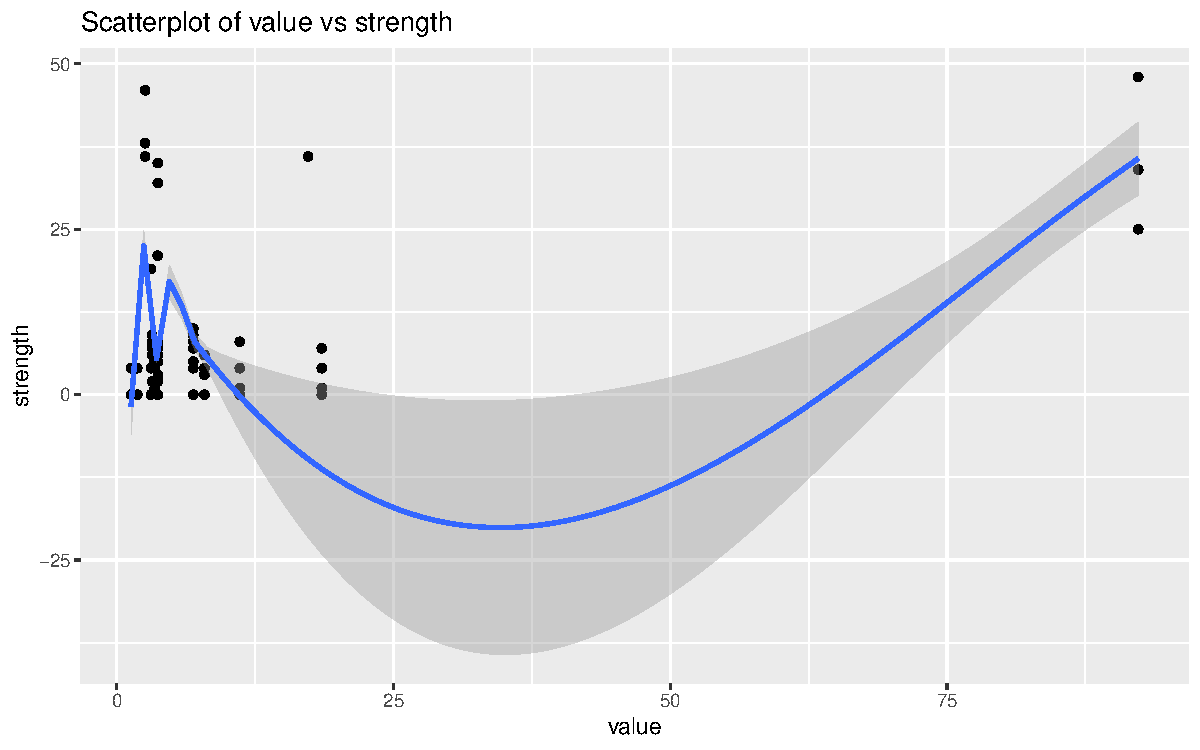
\includegraphics[width=0.8\linewidth]{Untitled_files/figure-beamer/scatterAttempt-1} \end{center}
\end{frame}

\hypertarget{conclusions}{%
\section{Conclusions}\label{conclusions}}

\begin{frame}{Conclusions}
\begin{itemize}
\tightlist
\item
  Name was the most common password category.
\item
  The time to crack some passwords took longer, regardless of what
  category.
\item
  There IS NO linear regression between rank and strength.
\item
  There IS a linear regression between strength and Time to crack.
\item
  There is NO linear regression between value and strength.
\end{itemize}
\end{frame}

\hypertarget{other-reccomendations}{%
\section{Other Reccomendations:}\label{other-reccomendations}}

\begin{frame}{Password Manager:}
\protect\hypertarget{password-manager}{}
\begin{itemize}
\tightlist
\item
  Minimises chances of password being guessed with RNG password
  generation.
\item
  Bitwarden changes the strength of the password.
\item
  Through our observation, this will make more unique passwords that
  would not be categorized. As we realise, that passwords categorised as
  a name I.e. Fluttershy is more common than a RNG one.
\end{itemize}
\end{frame}

\begin{frame}{References}
\protect\hypertarget{references}{}
Grilo, Ferreira, and Almeida (2021) Suo, Zhu, and Owen (2005) Hughes
(2020)

\hypertarget{refs}{}
\begin{CSLReferences}{1}{0}
\leavevmode\hypertarget{ref-grilo2021towards}{}%
Grilo, Miguel, João F Ferreira, and José Bacelar Almeida. 2021.
{``Towards Formal Verification of Password Generation Algorithms Used in
Password Managers.''} \emph{arXiv Preprint arXiv:2106.03626}.

\leavevmode\hypertarget{ref-tidyTuesday}{}%
Hughes, Ellis. 2020. \emph{tidytuesdayR: Access the Weekly 'TidyTuesday'
Project Dataset}. \url{https://CRAN.R-project.org/package=tidytuesdayR}.

\leavevmode\hypertarget{ref-suo2005graphical}{}%
Suo, Xiaoyuan, Ying Zhu, and G Scott Owen. 2005. {``Graphical Passwords:
A Survey.''} In \emph{21st Annual Computer Security Applications
Conference (ACSAC'05)}, 10--pp. IEEE.

\end{CSLReferences}
\end{frame}




\end{document}
